\documentclass[tikz,border=5pt]{standalone}
\usepackage{amsmath,amssymb,fontspec,unicode-math}
\setmainfont{STIXTwoText-Regular.otf}
\setmathfont{STIXTwoMath-Regular.otf}
\usetikzlibrary{positioning,arrows.meta,calc,decorations.pathreplacing}
\definecolor{hmtgray}{gray}{0.3}
\definecolor{hmtblue}{gray}{0.15}
\definecolor{hmtgold}{gray}{0.3}
\definecolor{hmtgreen}{gray}{0.1}
\definecolor{hmtred}{gray}{0.25}
\definecolor{hmtlightblue}{gray}{0.92}
\definecolor{hmtlightgold}{gray}{0.83}
\definecolor{hmtlightgreen}{gray}{0.97}
\definecolor{hmtlightred}{gray}{0.73}
\begin{document}
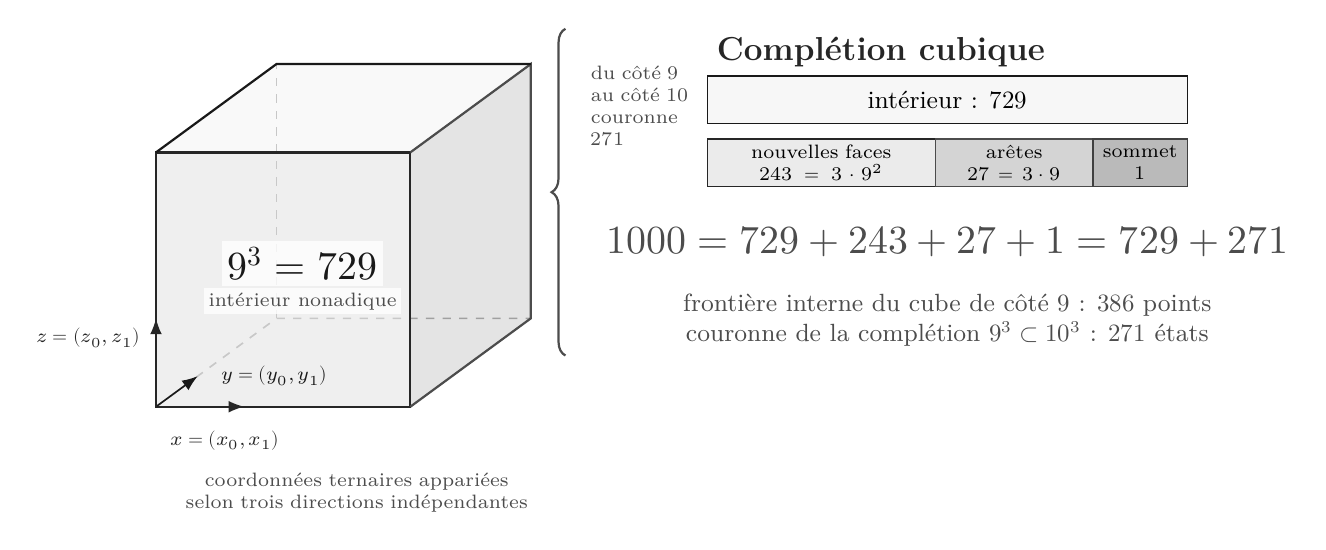
\begin{tikzpicture}[font=\small]
  \begin{scope}[x={(.95cm,0cm)},y={(.45cm,.33cm)},z={(0cm,.95cm)}]
  \coordinate (O) at (0,0,0);
  \coordinate (X) at (3.4,0,0);
  \coordinate (Y) at (0,3.4,0);
  \coordinate (XY) at (3.4,3.4,0);
  \coordinate (Z) at (0,0,3.4);
  \coordinate (XZ) at (3.4,0,3.4);
  \coordinate (YZ) at (0,3.4,3.4);
  \coordinate (XYZ) at (3.4,3.4,3.4);
  \draw[hmtgray,dashed,semithick] (O)--(Y)--(XY);
  \draw[hmtgray,dashed,semithick] (Y)--(YZ);
  \path[fill=hmtlightblue,fill opacity=.78]
    (O)--(X)--(XZ)--(Z)--cycle;
  \path[fill=hmtlightgold,fill opacity=.62]
    (X)--(XY)--(XYZ)--(XZ)--cycle;
  \path[fill=hmtlightgreen,fill opacity=.72]
    (Z)--(XZ)--(XYZ)--(YZ)--cycle;
  \draw[hmtblue,thick] (O)--(X)--(XZ)--(Z)--cycle;
  \draw[hmtgold,thick] (X)--(XY)--(XYZ)--(XZ);
  \draw[hmtgreen,thick] (Z)--(YZ)--(XYZ);
  \node[font=\bfseries\Large,hmtgreen,fill=white,fill opacity=.78,
    text opacity=1,inner sep=2pt] at (1.7,.55,1.72) {\(9^3=729\)};
  \node[font=\scriptsize,hmtgray,fill=white,fill opacity=.78,
    text opacity=1,inner sep=1.5pt] at (1.7,.55,1.22)
    {intérieur nonadique};
  \draw[-{Latex[length=2mm]},hmtblue,semithick]
    (O) -- (1.18,0,0)
    node[pos=.78,below=5pt,font=\scriptsize] {\(x=(x_0,x_1)\)};
  \draw[-{Latex[length=2mm]},hmtgreen,semithick]
    (O) -- (0,1.18,0)
    node[pos=1,right=5pt,font=\scriptsize] {\(y=(y_0,y_1)\)};
  \draw[-{Latex[length=2mm]},hmtblue,semithick]
    (O) -- (0,0,1.18)
    node[pos=.78,left=2pt,font=\scriptsize] {\(z=(z_0,z_1)\)};
  \end{scope}
  \node[align=center,text width=5.2cm,font=\scriptsize,hmtgray,
    anchor=north] at (2.55,-.72)
    {coordonnées ternaires appariées selon trois directions indépendantes};
  \draw[decorate,decoration={brace,amplitude=5pt},hmtgold,thick]
    (5.20,.65)--(5.20,4.80);
  \node[anchor=west,align=left,text width=1.25cm,font=\scriptsize,hmtgold]
    at (5.40,3.82) {du côté \(9\) au côté \(10\)\\couronne \(271\)};
  \begin{scope}[xshift=7cm,yshift=.45cm]
    \node[anchor=west,font=\bfseries\large,hmtblue] at (0,4.05)
      {Complétion cubique};
    \draw[fill=hmtlightgreen,draw=hmtgreen] (0,3.15) rectangle (6.1,3.75);
    \node at (3.05,3.45) {intérieur : \(729\)};
    \draw[fill=hmtlightblue,draw=hmtblue] (0,2.35) rectangle (2.9,2.95);
    \node[align=center,text width=2.75cm,font=\scriptsize] at (1.45,2.65)
      {nouvelles faces\\\(243=3\cdot9^2\)};
    \draw[fill=hmtlightgold,draw=hmtgold] (2.9,2.35) rectangle (4.9,2.95);
    \node[align=center,text width=1.8cm,font=\scriptsize] at (3.9,2.65)
      {arêtes\\\(27=3\cdot9\)};
    \draw[fill=hmtlightred,draw=hmtred] (4.9,2.35) rectangle (6.1,2.95);
    \node[align=center,font=\scriptsize] at (5.5,2.65)
      {sommet\\\(1\)};
    \node[font=\bfseries\Large,hmtgold] at (3.05,1.65)
      {\(1000=729+243+27+1=729+271\)};
    \node[align=center,hmtgray] at (3.05,.65)
      {frontière interne du cube de côté \(9\) : \(386\) points\\
       couronne de la complétion \(9^3\subset10^3\) : \(271\) états};
  \end{scope}
\end{tikzpicture}
\end{document}

